\newpage
\section*{Document réponse}
\begin{center}
\begin{tabular}{p{0.15\textwidth}p{0.15\textwidth}|p{0.15\textwidth}p{0.15\textwidth}|p{0.15\textwidth}p{0.15\textwidth}}
\textbf{Nom : } & &
\textbf{Prénom : } &  &
\textbf{Classe : } &  \\
\hline
\end{tabular}
\end{center}

\begin{figure}[H]
\centering
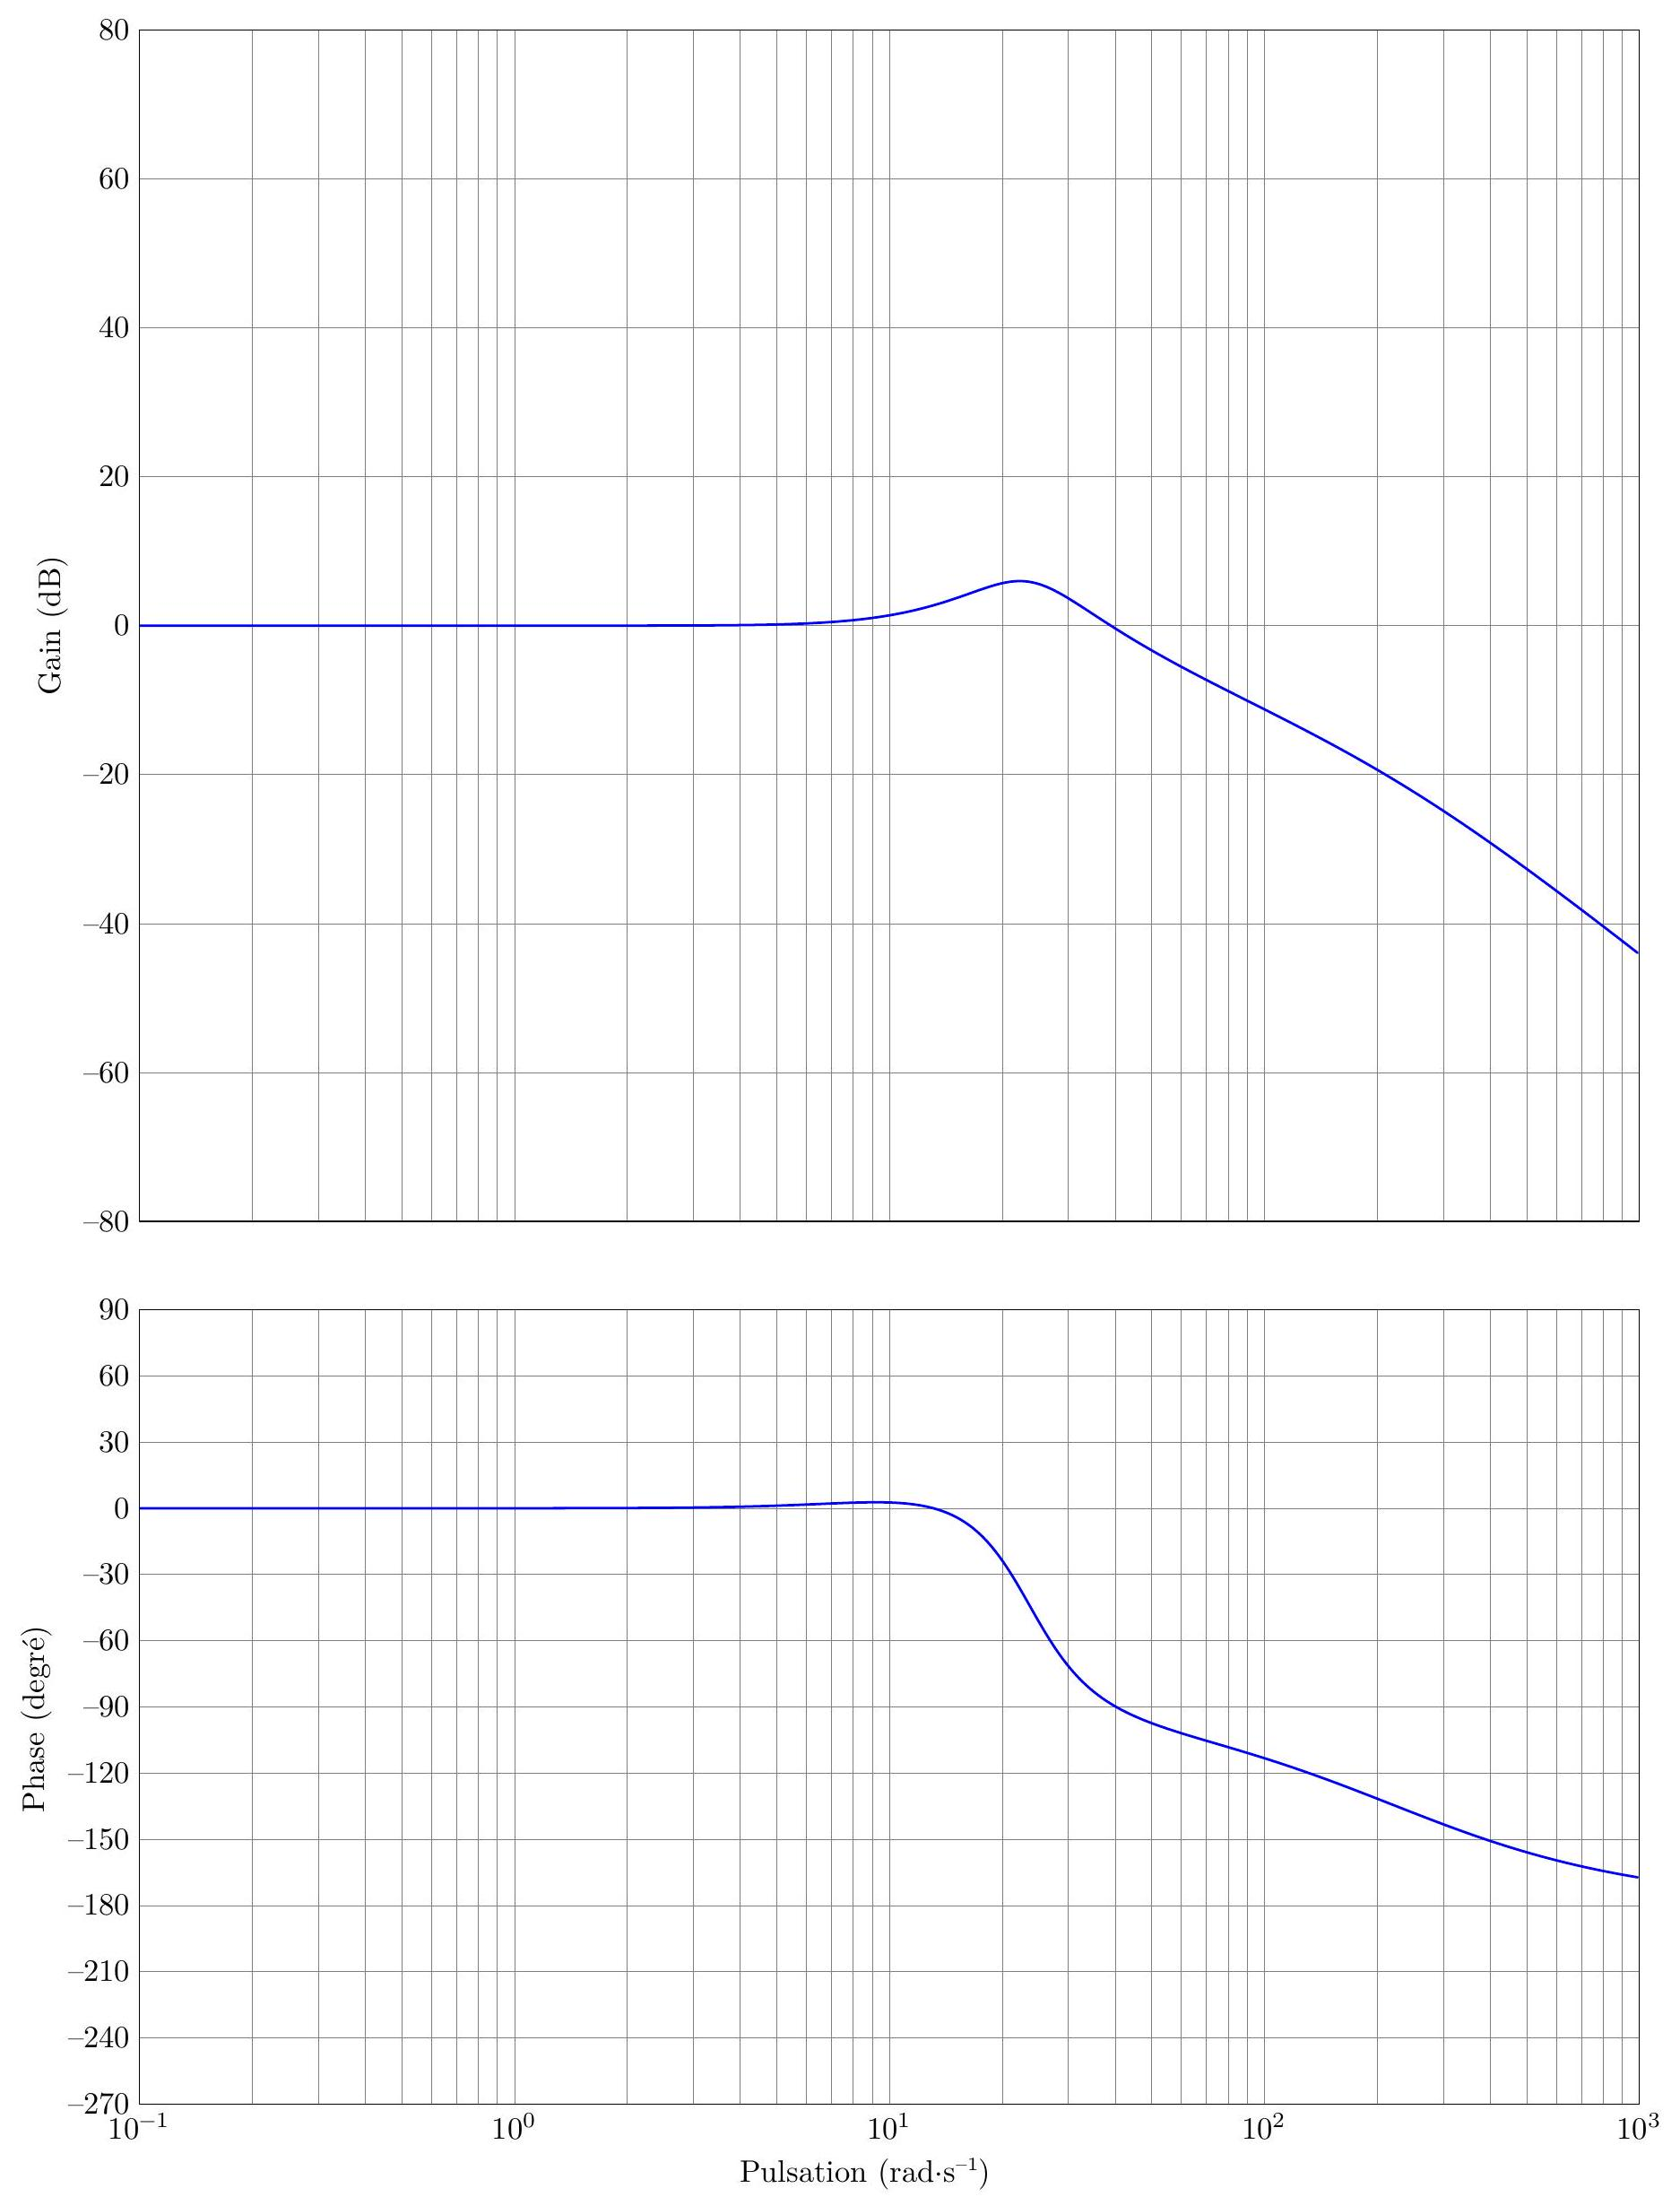
\includegraphics[width=\textwidth]{fig_18.jpg}
\caption{\label{fig:C} Diagrammes de Bode de la fonction $H(p)$ }%Extrait de l'aide sur la fonction Python \texttt{scipy.integrate.odeint} (Questions \ref{q:24} et \ref{q:25})}
\end{figure}


%\newpage
%
%\begin{tabular}{p{0.9\textwidth}}
%\\
%\hline
%\\
%\end{tabular}
%
%\newpage
%
%\begin{tabular}{p{0.9\textwidth}}
%\\
%\hline
%\\
%\end{tabular}
%
%\newpage
%
%\begin{tabular}{p{0.9\textwidth}}
%\\
%\hline
%\\
%\end{tabular}